% \documentclass[tikz,convert={outfile=\jobname.svg}]{standalone}
\documentclass[tikz]{standalone}
\usepackage{tikz}
\usetikzlibrary{fit,positioning, arrows, intersections}
\usepackage{verbatim}
\begin{document}
\centering
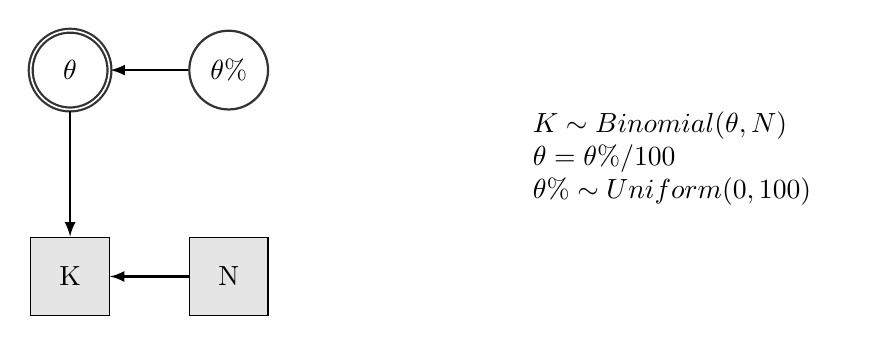
\begin{tikzpicture}
\tikzstyle{main}=[circle, minimum size = 10mm, thick, draw =black!80, node distance = 16mm]
\tikzstyle{connect}=[-latex, thick]
\tikzstyle{box}=[rectangle, draw=black!100, minimum size=10mm]

% 2. Nodes
%%%%%%%%%%
\node[box, fill=black!10] (K) {K};
\node[box, fill=black!10] (N) [right=of K] {N};
\node[main, fill=white!100, double] (theta) [above=of K] {$\theta$};
\node[main, fill=white!100] (ptheta) [above=of N] {$\theta \%$}; 
\node [anchor=east, text width=4cm] (dists) at (10, 1.5) {
          $K \sim Binomial(\theta, N)$\\
          $\theta = \theta \% / 100$ \\
          $\theta \% \sim Uniform(0, 100)$};
% 3. Arrows
%%%%%%%%%%%
\path (N)      edge [connect] (K)
      (theta)  edge [connect] (K)
      (ptheta) edge [connect] (theta);

\end{tikzpicture}

\end{document}